% Carried over verbatim from monograph/main.tex (Study 1 record, 13 Sep 2026).
\chapter{Executive overview}\label{s1:ch:ch01_executive_overview}

\section{The entire project in one page}

The initial problem was simple to state: \emph{when a benchmark calls every image file an independent example, is that file really the unit that was independently sampled?} In cervical cytology, the answer can be no. One microscope field can emit several cell crops. If those crops are split independently, their source field can appear on both sides of evaluation.

The project followed a staged answer:
\begin{enumerate}[leftmargin=2em]
  \item define the independent parent unit for four public datasets;
  \item recover exact crop-to-parent mappings, using independent recovery branches where the release permits them;
  \item refuse downstream analysis unless agreement, geometry, counts, and uniqueness pass;
  \item calculate how often random crop splitting separates siblings;
  \item detect literal pixel overlap and conservative cross-parent near-duplicate components;
  \item create four fixed protocols that isolate independence from training-set size;
  \item ask whether parent identity is visually learnable after removing candidate cues;
  \item re-run multiple classifier and segmentation families over five fixed seeds;
  \item use paired inference, effect sizes, bootstrap intervals, and declared BH families;
  \item preserve failed attempts and execution amendments rather than erasing them.
\end{enumerate}

\begin{figure}[H]
\centering
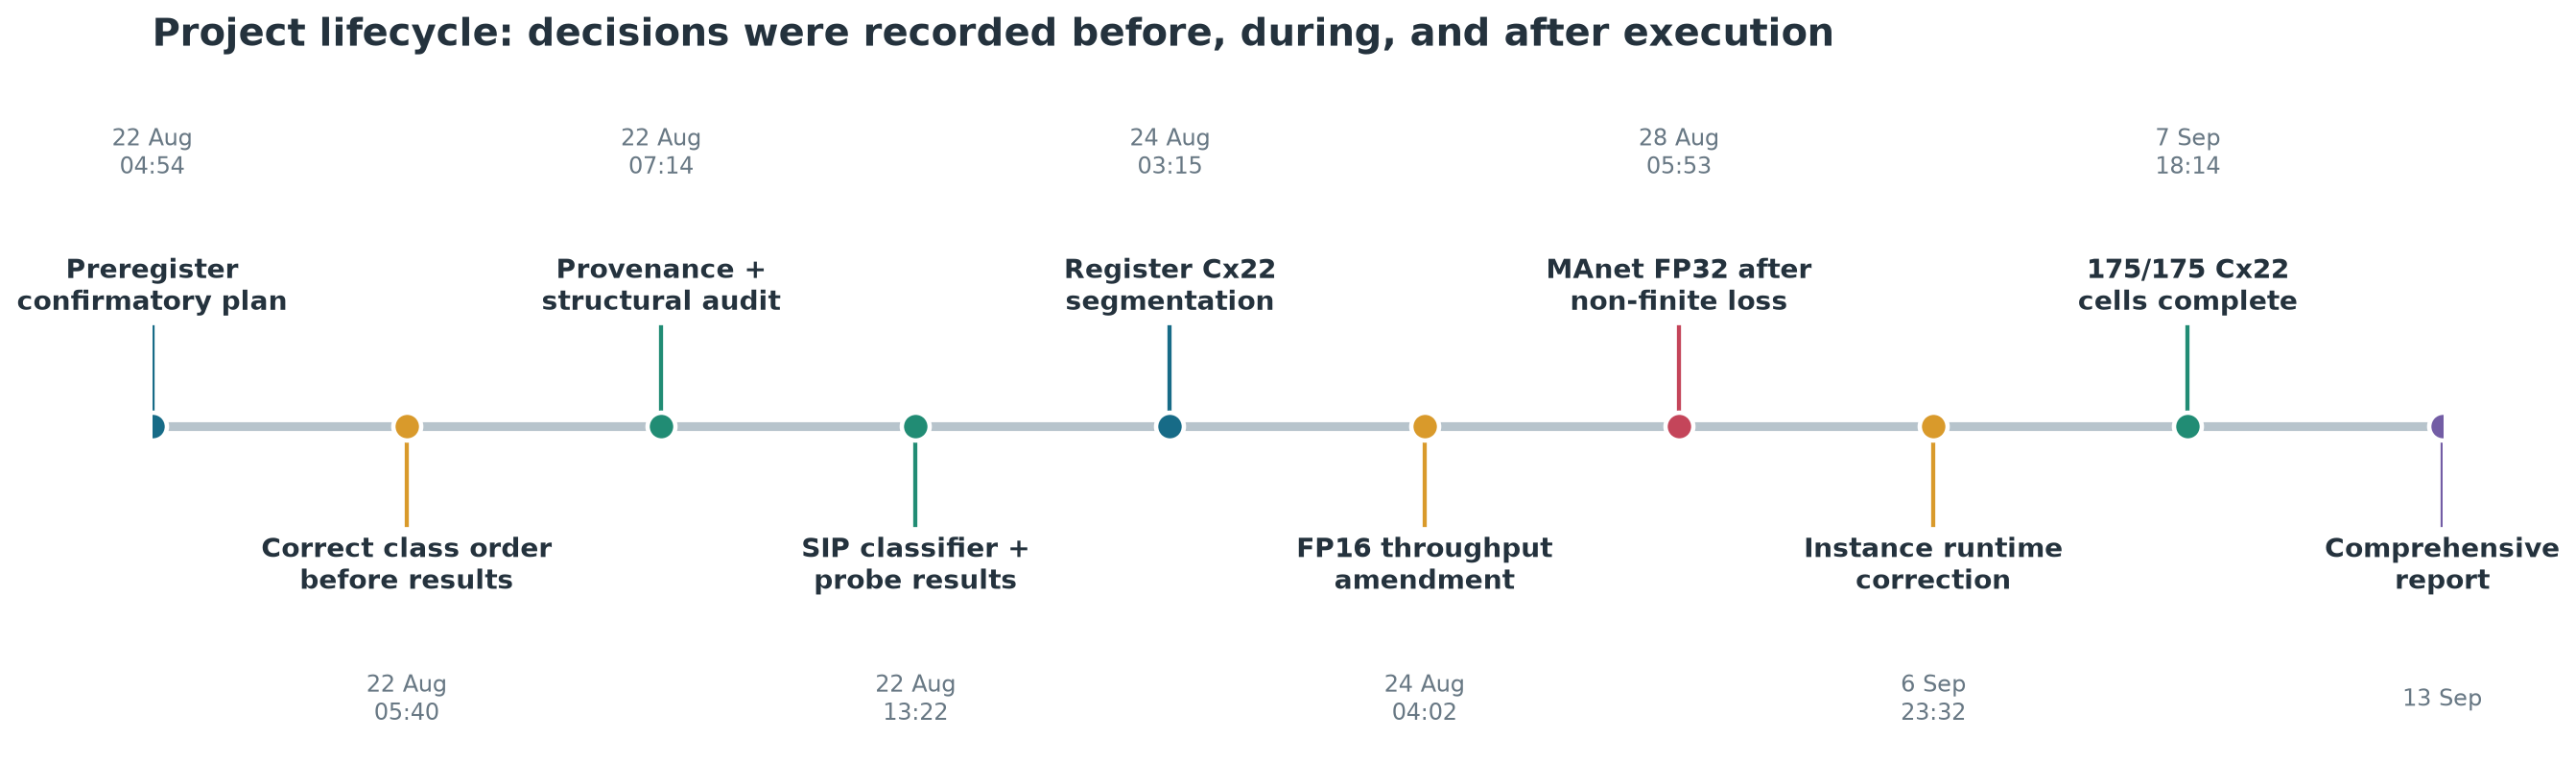
\includegraphics[width=\textwidth]{lifecycle_timeline.png}
\caption{The project lifecycle. Blue events register decisions, green events record completed evidence, gold events document execution-driven amendments, red records a numerical failure, and purple marks this report.}
\label{s1:fig:lifecycle}
\end{figure}

\section{Headline findings, without spin}

\begin{longtable}{p{0.22\textwidth}p{0.19\textwidth}p{0.51\textwidth}}
\caption{Headline conclusions and their correct strength.}\label{s1:tab:headline}\\
\toprule
Question & Answer & Evidence and boundary \\
\midrule
\endfirsthead
\toprule
Question & Answer & Evidence and boundary \\
\midrule
\endhead
\bottomrule
\endfoot
Can provenance be recovered? & Yes & SIPaKMeD branches agree on 4,049/4,049 crops; all boxes are contained; all dataset and class totals match. \\
Does random crop splitting share parents? & Yes & Mean P1 test-parent overlap is 92.62\% on SIPaKMeD, 85.23\% on Cx22, and 99.97\% on CRIC. \\
Does the negative control remain negative? & Yes & Herlev has one released cell per parent and returns exactly 0.00\% structural leakage for all seeds. \\
Are literal pixels shared? & Yes, in SIPaKMeD P1 & 52.62\% of test crops share at least one source pixel with a training crop; P2/P3 return zero. \\
Is source identity learnable? & Yes & A 424-way ResNet-18 reaches 25.73\% versus 0.2358\% chance; shuffled labels return 0.17\% and cover chance. \\
Is P1 accuracy universally inflated? & Not established & All six SIPaKMeD and all seven Cx22 P1--P2 means are positive, but no contrast survives BH correction. \\
Does stronger grouping always lower score? & No & SIPaKMeD's registered P3 $\leq$ P2 $\leq$ P1 model ordering fails for four of six architectures. The failure is retained. \\
Is Cx22's official split defective? & No such claim & The authors' Multi-Train/Multi-Test parent sets are disjoint. The pooled stress test asks what happens under a different downstream reuse pattern. \\
Is the release fully ready? & Not yet & The clean-clone/virgin-host evidence, lab-paper crosswalk, and independent Figure-1 reader gate remain pending. \\
\end{longtable}
